\documentclass{standalone}
\usepackage{tikz}
\usepackage{amsmath}
\usetikzlibrary{positioning, shapes.geometric, calc}

% This is just a box with labels - Simple
\tikzset{
        priority-arbiter/.style={
            regular polygon sides=4, draw, minimum size=3.0cm, very thick,
            label={[anchor=west,  yshift=1.0cm]   left: {\normalsize REQ\_0}},
            label={[anchor=west,  yshift=0.2cm]   left: {\normalsize REQ\_1}},
            label={[anchor=west,  yshift=-0.6cm]  left: {\normalsize REQ\_2}},
            label={[anchor=east,  yshift=1.0cm]   right:{\normalsize GNT\_0}},
            label={[anchor=east,  yshift=0.2cm]   right:{\normalsize GNT\_1}},
            label={[anchor=east,  yshift=-0.6cm]  right:{\normalsize GNT\_2}},
            label={[anchor=south, xshift=-0.5cm]  below:{\normalsize CLK}},
            label={[anchor=south, xshift=0.5cm]   below:{\normalsize RST}}
        },
}

\begin{document}

 \resizebox{10cm}{9cm}{

    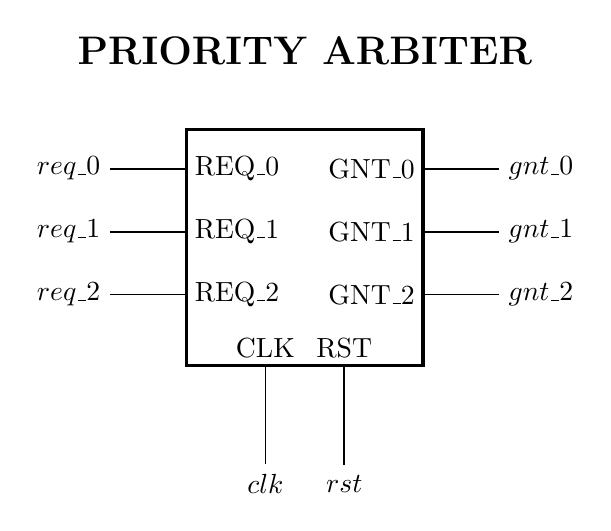
\begin{tikzpicture}[node distance=.2cm]

        % DRAW NODES (I like to do them relative to each other)
        \node[priority-arbiter] (PA)   at (0,0)                  {};
        \node[]                 (REQ0) at ($(PA)+(-3.0,1.0)$)    {\normalsize $req\_0$};
        \node[]                 (REQ1) at ($(PA)+(-3.0,0.2)$)    {\normalsize $req\_1$};
        \node[]                 (REQ2) at ($(PA)+(-3.0,-0.6)$)   {\normalsize $req\_2$};
        \node[]                 (GNT0) at ($(PA)+(3.0,1.0)$)     {\normalsize $gnt\_0$};
        \node[]                 (GNT1) at ($(PA)+(3.0,0.2)$)     {\normalsize $gnt\_1$};
        \node[]                 (GNT2) at ($(PA)+(3.0,-0.6)$)    {\normalsize $gnt\_2$};
        \node[]                 (CLK)  at ($(PA)+(-0.5,-3.0)$)   {\normalsize $clk$};
        \node[]                 (RST)  at ($(PA)+(0.5,-3.0)$)    {\normalsize $rst$};
        \node[]                 (NAME) at ($(PA)+(0, 2.5)$)      {\Large \textbf {PRIORITY ARBITER}};

        % CONNECT INPUTS
        \draw [semithick] (REQ0) -- ($(REQ0)+(1.5,0)$);
        \draw [semithick] (REQ1) -- ($(REQ1)+(1.5,0)$);
        \draw [semithick] (REQ2) -- ($(REQ2)+(1.5,0)$);

        % CONNECT OUTPUTS
        \draw [semithick] ($(GNT0)+(-1.5,0)$) -- (GNT0);
        \draw [semithick] ($(GNT1)+(-1.5,0)$) -- (GNT1);
        \draw [semithick] ($(GNT2)+(-1.5,0)$) -- (GNT2);
        
        % CONNECT CLK AND RST
        \draw [semithick] ($(CLK)+(0,1.5)$) -- (CLK);
        \draw [semithick] ($(RST)+(0,1.5)$) -- (RST);

    \end{tikzpicture}
}

\end{document} 
